\documentclass[dvipdfmx]{article}

\usepackage[top=30truemm,bottom=20truemm,left=25truemm,right=30truemm]{geometry}

\usepackage{enumerate}
\usepackage{tikz}
\usepackage{xcolor}
\usepackage{multicol}
\usepackage{mathtools}

\makeatletter

\renewcommand{\thetable}{
    \arabic{section}.\arabic{table}
}

\@addtoreset{table}{section}

\renewcommand{\thefigure}{
	\arabic{section}.\arabic{figure}
}

\@addtoreset{figure}{section}

\renewcommand{\theequation}{
	\arabic{section}.\arabic{equation}
}

\@addtoreset{equation}{section}%

\makeatother

\title{Binary tree}
\author{Masaki Nakata}

\begin{document}
\maketitle

\section{Binary tree}
I explain my implementation of the binarytree. I discuss the insert function, and then the search function, and finally the delete function. 
\begin{enumerate}
\item {\bf insert}\\
  We need the former binary tree and the number or object to insert for inserting the object. For constitution for the binary tree, we have to set up a root, but if we distinguish it between nodes, we must have much more functions. So, I define the parent of the root is the atom called ``head''. A insert function as a graph means seeing the binary tree like a subtree under the atom which work as a insert and changing a subtree. The end of a subtree like a leaf will be changed a null node to the node which means a number. In the first place, we hangle the binary tree as follows.
  \begin{figure}[ht]
    \begin{center}
      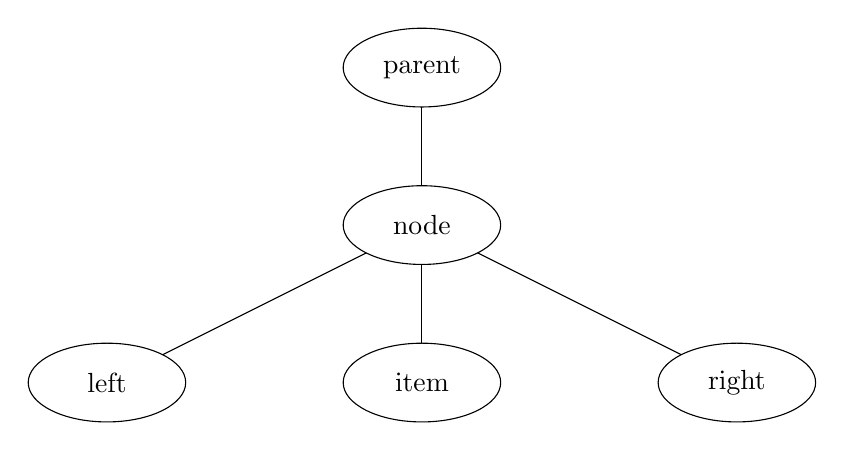
\begin{tikzpicture}[>=stealth]
        \draw (0,0)--(0,-4);
        \draw (0,-2)--(4,-4);
        \draw (0,-2)--(-4,-4);
        
        \draw[fill=white,xscale=2] (0,0) circle [radius=0.5];
        \draw[fill=white,xscale=2] (0,-2) circle [radius=0.5];
        \draw[fill=white,xscale=2] (0,-4) circle [radius=0.5];
        
        \draw[fill=white,xscale=2] (2,-4) circle[radius=0.5];
        \draw[fill=white,xscale=2] (-2,-4) circle[radius=0.5];
        
        \node at (0,0) {parent};
        \node at (0,-2) {node};
        \node at (0,-4) {item};
        \node at (-4,-4) {left};
        \node at (4,-4) {right};
      \end{tikzpicture}
    \end{center}
    \caption{node composition}
  \end{figure}
  
  ``Parent'' means the parent of the node and it is only one and it should be a node or the head atom. And ``left'' means a child node of a node and it is a null node or a node which has the key less than the  key of the node. As well, a ``right'' node is a null node or a node which has the key more than the key of the node. Finally, ``item'' is a key of a node and it is a number or a object. In this time, I deal with a object as number. So, a node connects five nodes (we can regard that a node connects five atoms). In implementing by LMNtal, we can use (or think) atoms and links are same(correctly wrong). The link connected to the parent is {\ttfamily P}, and the one of the item is {\ttfamily X}, the left one is {\ttfamily L}, and the right one is {\ttfamily R}. So, I define the node atom and links connected it as follows.
  \begin{center}
    {\ttfamily node(P, X, L, R)}  $\ \coloneqq \ node(parent,\ items(key),\ left,\ right)$
  \end{center}
  About the timing of insertion, there are two possible scenarios: being in a node which has the key and works as a leaf, or being in a null node. If I implement the insert function when the insertion atom is in a node which has the key, we can three patterns. It's possible that a node which works as a leaf has no children, or only child on the right, or only child on the left. So, we have to implement three functions for inserting at the leaf. But, the less we can implement functions, the easier it is to see the program. Hence, I chose the implementation in a null node.
  \begin{figure}[ht]
    \begin{multicols}{2}
      \begin{center}
        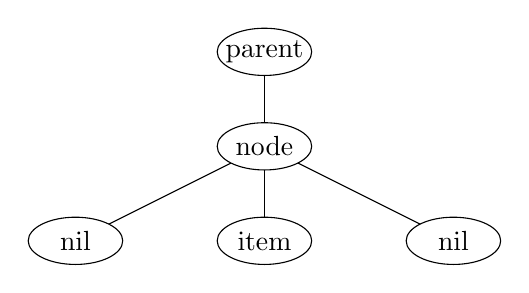
\begin{tikzpicture}[>=stealth,scale=0.6]
          \draw (0,0)--(0,-4);
          \draw (0,-2)--(4,-4);
          \draw (0,-2)--(-4,-4);
          
          \draw[fill=white,xscale=2] (0,0) circle [radius=0.5];
          \draw[fill=white,xscale=2] (0,-2) circle [radius=0.5];
          \draw[fill=white,xscale=2] (0,-4) circle [radius=0.5];
          
          \draw[fill=white,xscale=2] (2,-4) circle[radius=0.5];
          \draw[fill=white,xscale=2] (-2,-4) circle[radius=0.5];
          
          \node at (0,0) {parent};
          \node at (0,-2) {node};
          \node at (0,-4) {item};
          \node at (-4,-4) {nil};
          \node at (4,-4) {nil};
        \end{tikzpicture}
      \end{center}
      \begin{center}
        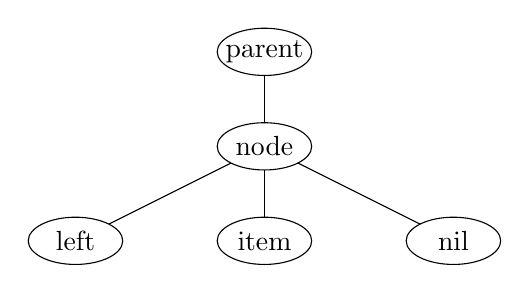
\begin{tikzpicture}[>=stealth,scale=0.6]
          \draw (0,0)--(0,-4);
          \draw (0,-2)--(4,-4);
          \draw (0,-2)--(-4,-4);
          
          \draw[fill=white,xscale=2] (0,0) circle [radius=0.5];
          \draw[fill=white,xscale=2] (0,-2) circle [radius=0.5];
          \draw[fill=white,xscale=2] (0,-4) circle [radius=0.5];
          
          \draw[fill=white,xscale=2] (2,-4) circle[radius=0.5];
          \draw[fill=white,xscale=2] (-2,-4) circle[radius=0.5];
          
          \node at (0,0) {parent};
          \node at (0,-2) {node};
          \node at (0,-4) {item};
          \node at (-4,-4) {left};
          \node at (4,-4) {nil};
        \end{tikzpicture}
      \end{center}
      \begin{center}
        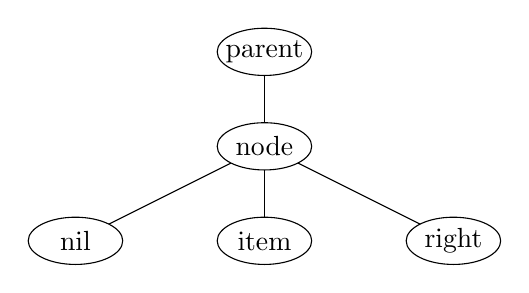
\begin{tikzpicture}[>=stealth,scale=0.6]
          \draw (0,0)--(0,-4);
          \draw (0,-2)--(4,-4);
          \draw (0,-2)--(-4,-4);
          
          \draw[fill=white,xscale=2] (0,0) circle [radius=0.5];
          \draw[fill=white,xscale=2] (0,-2) circle [radius=0.5];
          \draw[fill=white,xscale=2] (0,-4) circle [radius=0.5];
          
          \draw[fill=white,xscale=2] (2,-4) circle[radius=0.5];
          \draw[fill=white,xscale=2] (-2,-4) circle[radius=0.5];
          
          \node at (0,0) {parent};
          \node at (0,-2) {node};
          \node at (0,-4) {item};
          \node at (-4,-4) {nil};
          \node at (4,-4) {right};
        \end{tikzpicture}
      \end{center}
    \end{multicols}
    \caption{leaf composition}
  \end{figure}

  A null node can be implemented as below.
  \begin{center}
    {\ttfamily nil(P)} $\ \coloneqq\ nullnode(parent)$
  \end{center}
  As I mentioned at the beginning, the insert function only looks at the subtree. So, the composition on the graph is as follows.
  \begin{figure}[ht]
    \begin{center}
      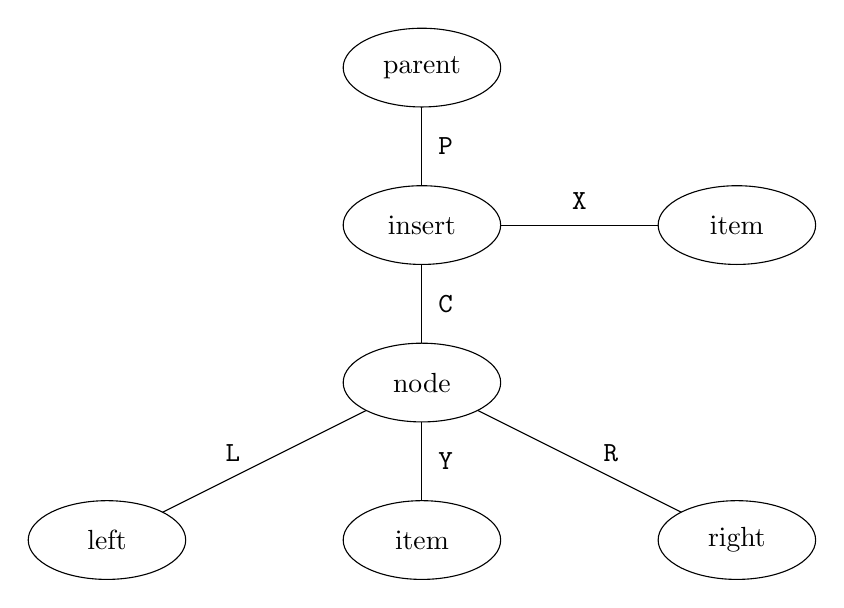
\begin{tikzpicture}[>=stealth]
        \draw (0,2)--(0,-4);
        \draw (0,0)--(4,0);
        \draw (0,-2)--(4,-4);
        \draw (0,-2)--(-4,-4);

        \draw[fill=white,xscale=2] (0,2) circle [radius=0.5];
        \draw[fill=white,xscale=2] (0,0) circle [radius=0.5];
        \draw[fill=white,xscale=2] (0,-2) circle [radius=0.5];
        \draw[fill=white,xscale=2] (0,-4) circle [radius=0.5];

        \draw[fill=white,xscale=2] (2,0) circle[radius=0.5];
        
        \draw[fill=white,xscale=2] (2,-4) circle[radius=0.5];
        \draw[fill=white,xscale=2] (-2,-4) circle[radius=0.5];

        \node at (0,2) {parent};
        \node at (0,0) {insert};
        \node at (0,-2) {node};
        \node at (0,-4) {item};
        \node at (-4,-4) {left};
        \node at (4,-4) {right};
        \node at (4,0) {item};

        \node at (0.3,1) {\ttfamily P};
        \node at (0.3,-1) {\ttfamily C};
        \node at (2,0.3) {\ttfamily X};
        \node at (0.3, -3) {\ttfamily Y};
        \node at (-2.4,-2.9) {\ttfamily L};
        \node at (2.4, -2.9) {\ttfamily R};
      \end{tikzpicture}
    \end{center}
    \caption{the insert function as the graph}
    \label{insert function}
  \end{figure}
  
  Look at figure \ref{insert function}, we can use to compare the link name as the values of atoms connected to the link in LMNtal. Therefore {\ttfamily X} is treated as the key of insertion and {\ttfamily Y} is treated as the node key. If {\ttfamily X} is bigger than {\ttfamily Y}, the atom of the insertion moves the right subtree and the parent of insertion will be changed to node which has link {\ttfamily Y}. Also we can think as well when {\ttfamily X} is smaller than {\ttfamily Y}.

  
\end{enumerate}
\end{document}
